\begin{figure}[thpb]
    \centering
        \begin{subfigure}{0.49\linewidth}
		\centering
		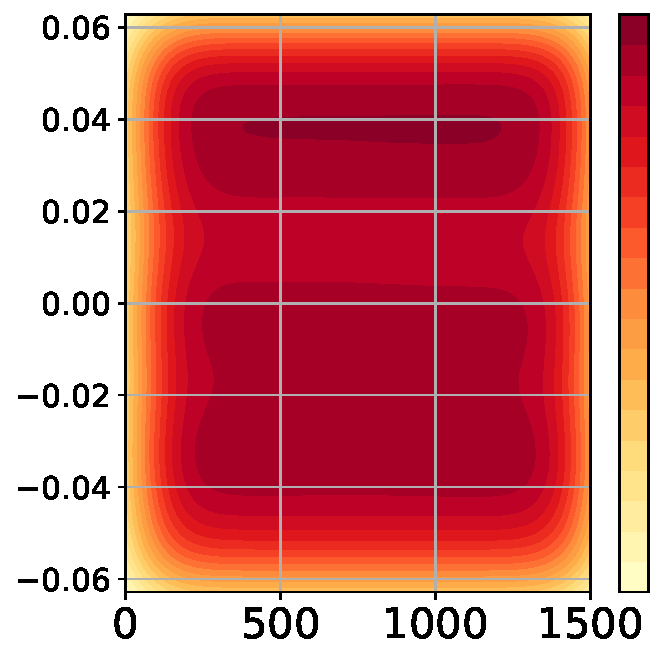
\includegraphics[width=1.0\linewidth]{fig/weight_echo/Para_a.pdf}
		\caption{Distribution of parameter $\boldsymbol{\alpha}_t$. Darker regions indicate higher density.} 
		\label{fig:wei:para_a:echo}
	\end{subfigure}
        %
	\begin{subfigure}{0.49\linewidth}
		\centering
		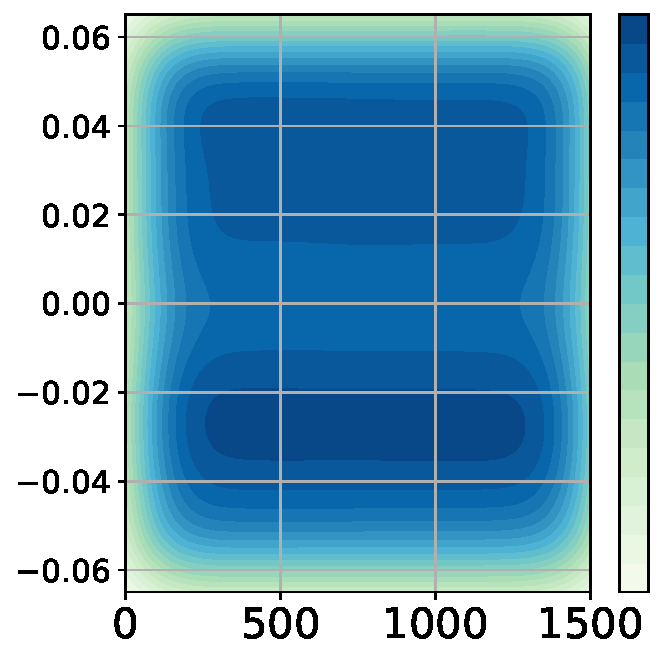
\includegraphics[width=1.0\linewidth]{fig/weight_echo/Para_b.pdf}
		\caption{Distribution of parameter $\boldsymbol{\beta}_t$. Darker regions indicate higher density.} 
		\label{fig:wei:para_b:echo}
	\end{subfigure}
	%\qquad
	\begin{subfigure}{0.49\linewidth}
		\centering
		
\includegraphics[width=1.0\linewidth]{fig/weight_echo/Grad_a_b.pdf}
		\caption{Distribution of gradient $\boldsymbol{\alpha}_t$ and $\boldsymbol{\beta}_t$.}
		\label{fig:wei:Grad:echo}
	\end{subfigure}
        \hspace{0.03mm}
	\begin{subfigure}{0.49\linewidth}
		\centering
		\includegraphics[width=1.0\linewidth]{fig/weight_echo/person_Grad_a_b.pdf}
		\caption{Pearson Correlation of gradient $\boldsymbol{\alpha}_t$ and $\boldsymbol{\beta}_t$. }
		\label{fig:wei:person:echo}
	\end{subfigure}
    \caption{Weights of parameters $\boldsymbol{\alpha}_t$ and $\boldsymbol{\beta}_t$ over training steps on EchoNet-Dynamic.}
    \label{fig:wei:echo}
\end{figure}